\documentclass[12pt, a4paper]{article}
\usepackage[utf8]{inputenc}
\usepackage[T1]{fontenc}
\usepackage[french]{babel}
\usepackage{graphicx}
\usepackage{hyperref}
\usepackage{geometry}
\usepackage{listings}
\usepackage{xcolor}
\geometry{hmargin=2cm, vmargin=2cm}

\lstdefinelanguage{JavaScript}{
  keywords={const, let, var, if, else, for, while, return, function, true, false, require, module, exports, async, await, new, try, catch, throw},
  keywordstyle=\color{blue}\bfseries,
  ndkeywords={class, export, boolean, implements, import, this},
  ndkeywordstyle=\color{teal}\bfseries,
  identifierstyle=\color{black},
  sensitive=false,
  comment=[l]{//},
  morecomment=[s]{/*}{*/},
  commentstyle=\color{green!60!black}\ttfamily,
  stringstyle=\color{red}\ttfamily,
  morestring=[b]',
  morestring=[b]"
}

\lstset{
    language=JavaScript,
    backgroundcolor=\color{black!5},
    basicstyle=\ttfamily\footnotesize,
    keywordstyle=\color{blue}\bfseries,
    stringstyle=\color{red},
    commentstyle=\color{green!60!black},
    numbers=left,
    numberstyle=\tiny\color{gray},
    stepnumber=1,
    numbersep=8pt,
    showstringspaces=false,
    breaklines=true,
    frame=single,
    extendedchars=true,
    literate=
      {é}{{\'{e}}}1
      {è}{{\`{e}}}1
      {ê}{{\^{e}}}1
      {ë}{{\"e}}1
      {à}{{\`{a}}}1
      {â}{{\^{a}}}1
      {î}{{\^{i}}}1
      {ï}{{\"i}}1
      {ô}{{\^{o}}}1
      {û}{{\^{u}}}1
      {ù}{{\`{u}}}1
      {ç}{{\c{c}}}1
}

\title{\textbf{Compte-rendu du TP 4 : Authentification JWT \& Sécurité des Routes}}
\author{
    Réalisé par : \textbf{JOSEPH MUKUBU KAPOYA} \\
    \textit{5ème Datascience et IA, Groupe 1}
}
\date{\today}

\begin{document}
\maketitle

\section*{Introduction}
Ce quatrième atelier pratique fait évoluer notre API blog vers une architecture sécurisée de bout en bout grâce à l'\textbf{authentification JWT (JSON Web Token)} et au \textbf{contrôle d'accès basé sur les rôles (RBAC)}. Les données sont désormais protégées par des jetons cryptographiques : seuls les utilisateurs authentifiés peuvent créer, modifier ou supprimer des ressources, et seuls les administrateurs accèdent aux données sensibles.

Les objectifs pédagogiques de ce TP sont :
\begin{itemize}
    \item Hacher de manière irréversible les mots de passe avec \texttt{bcryptjs} (sel + hachage).
    \item Générer et vérifier des jetons JWT avec \texttt{jsonwebtoken}.
    \item Implémenter un middleware \texttt{protect} qui intercepte et valide chaque requête entrante.
    \item Appliquer le contrôle d'accès RBAC via \texttt{adminOnly}.
    \item Extraire l'identité de l'auteur depuis le token (et non du corps de la requête) pour garantir l'inviolabilité.
    \item Gérer les cas d'erreur : token absent, invalide, ou expiré (\texttt{TokenExpiredError}).
\end{itemize}

\section{Réponse argumentée à l'encadré « Prédisez »}

\subsection*{Problématique : Sécurité et identité de l'auteur d'un article}
\textbf{Question :} \textit{Pourquoi extraire l'identifiant de l'auteur depuis \texttt{req.user.\_id} (injecté par le middleware après vérification du JWT) plutôt que depuis \texttt{req.body.authorId} soumis par le client ?}

\textbf{Réponse argumentée :} \\
Il s'agit d'une distinction fondamentale entre \textbf{authentification} et \textbf{confiance accordée au client}.
\begin{enumerate}
    \item \textbf{Inviolabilité cryptographique :} Le JWT est signé avec \texttt{JWT\_SECRET}, une clé connue uniquement du serveur. La méthode \texttt{jwt.verify()} garantit que le contenu du token (notamment \texttt{id} et \texttt{role}) n'a pas été altéré. Toute tentative de falsification invalide la signature.
    \item \textbf{Usurpation d'identité via \texttt{req.body} :} Si l'auteur était fourni dans le corps de la requête, n'importe quel client malveillant pourrait envoyer l'ObjectId d'un autre utilisateur pour lui attribuer des articles à son insu — c'est une attaque de type \textbf{IDOR (Insecure Direct Object Reference)}.
    \item \textbf{Principe du moindre privilège :} En fixant \texttt{author: req.user.\_id} côté serveur, on applique le principe que le client ne fournit que les données métier (\texttt{title}, \texttt{content}), jamais son identité — qui est établie par le système d'authentification.
    \item \textbf{Audit et traçabilité :} Les actions sont associées à un compte vérifié et enregistré, rendant toute répudiation impossible.
\end{enumerate}

\section{Captures d'Écran des Tests Postman}

\subsection{Inscription d'un nouvel utilisateur}

\begin{figure}[htbp]
    \centering
    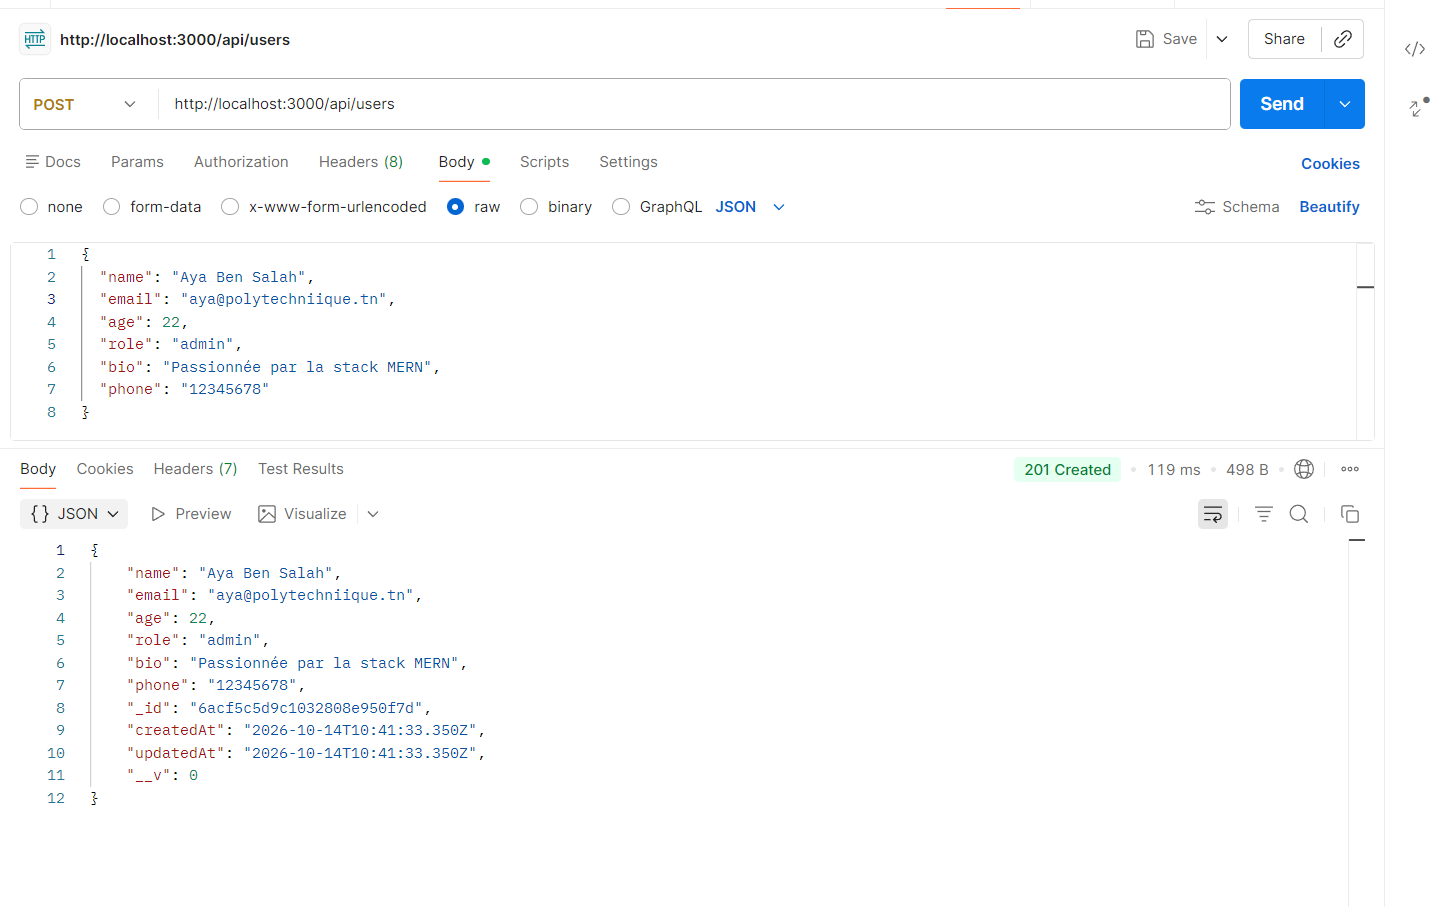
\includegraphics[width=0.78\textwidth]{postmanTP4-1.png}
    \caption{POST /api/users/register -- 201 Created (inscription réussie)}
    \vspace{0.1cm}
    \small \textit{Description :} Création d'un compte avec \texttt{name}, \texttt{email} et \texttt{password}. Le mot de passe est haché par \texttt{bcrypt} avant persistance. La réponse \textbf{201 Created} retourne l'objet utilisateur avec son \texttt{\_id}, \texttt{role} et un \textbf{JWT valide 24h}.
\end{figure}

\clearpage
\subsection{Connexion et récupération du JWT}

\begin{figure}[htbp]
    \centering
    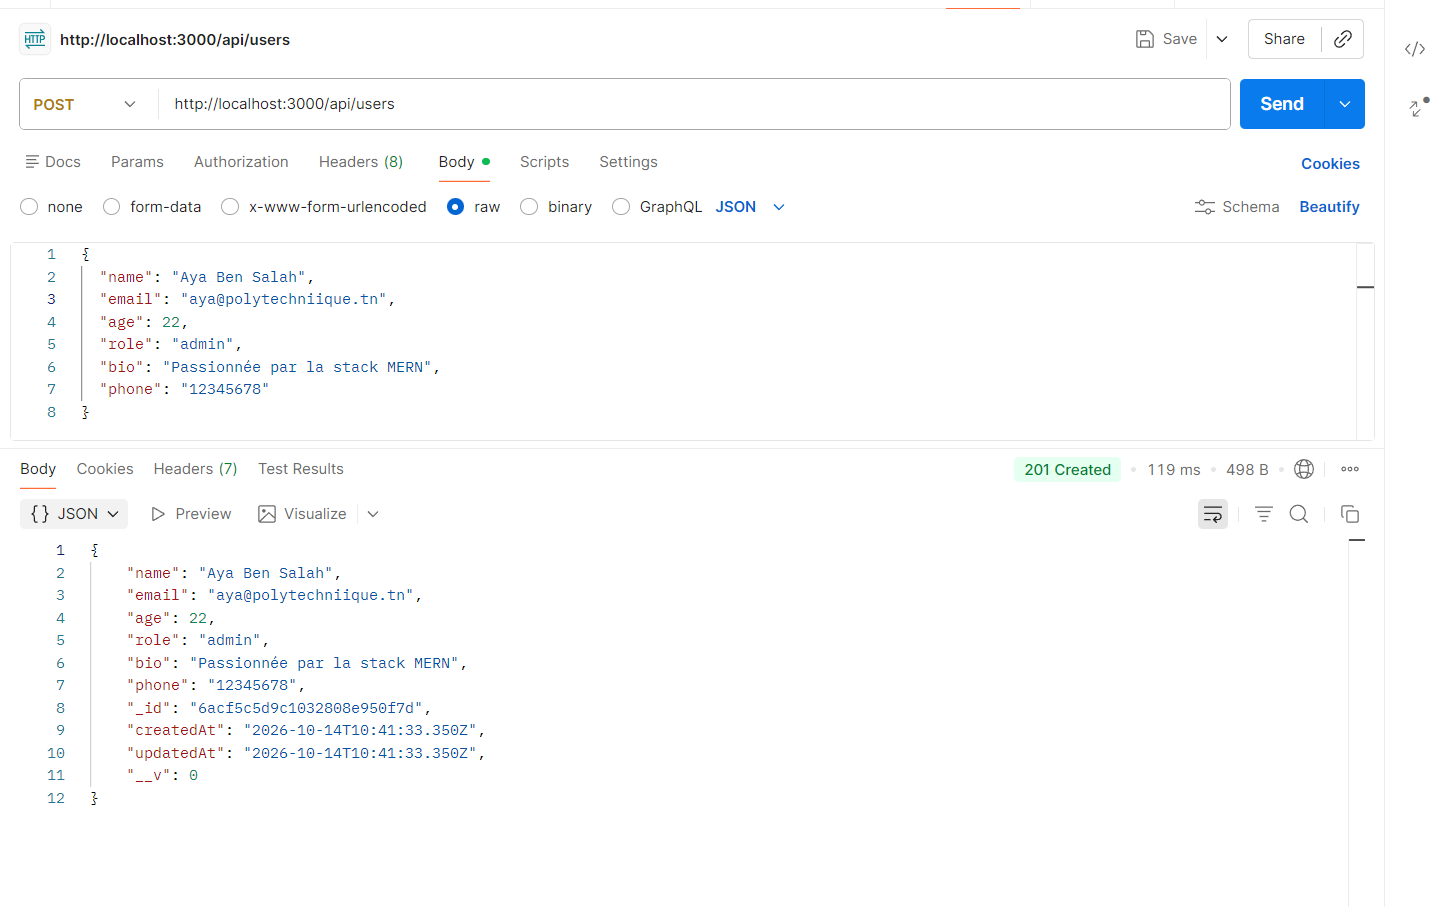
\includegraphics[width=0.78\textwidth]{postmanTP4-2.png}
    \caption{POST /api/users/login -- 200 OK (connexion et JWT)}
    \vspace{0.1cm}
    \small \textit{Description :} Authentification avec les identifiants valides. \texttt{bcrypt.compare()} vérifie le mot de passe en temps constant sans jamais déchiffrer le hash. La réponse \textbf{200 OK} retourne le token JWT à copier pour les requêtes protégées.
\end{figure}

\clearpage
\subsection{Rejet sans token -- 401 Unauthorized}

\begin{figure}[htbp]
    \centering
    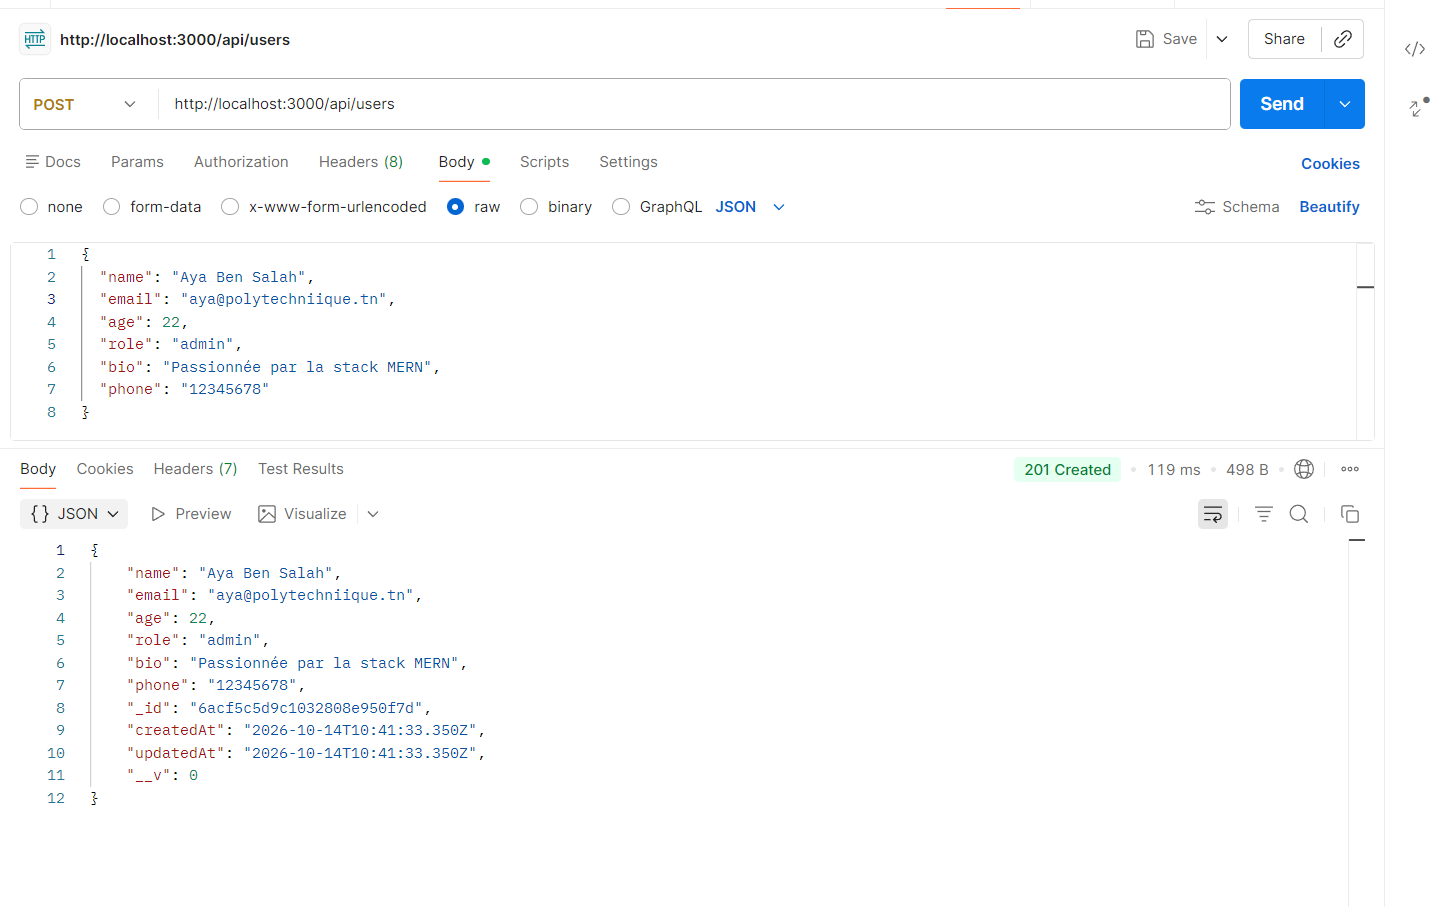
\includegraphics[width=0.78\textwidth]{postmanTP4-3.png}
    \caption{GET /api/users/profile -- 401 Unauthorized (aucun token fourni)}
    \vspace{0.1cm}
    \small \textit{Description :} Accès à la route protégée \texttt{/profile} sans en-tête \texttt{Authorization}. Le middleware \texttt{protect} détecte l'absence du header et renvoie immédiatement \textbf{401 Unauthorized} avec le message \texttt{"Non autorise, aucun token fourni"}.
\end{figure}

\clearpage
\subsection{Accès au profil avec token valide -- 200 OK}

\begin{figure}[htbp]
    \centering
    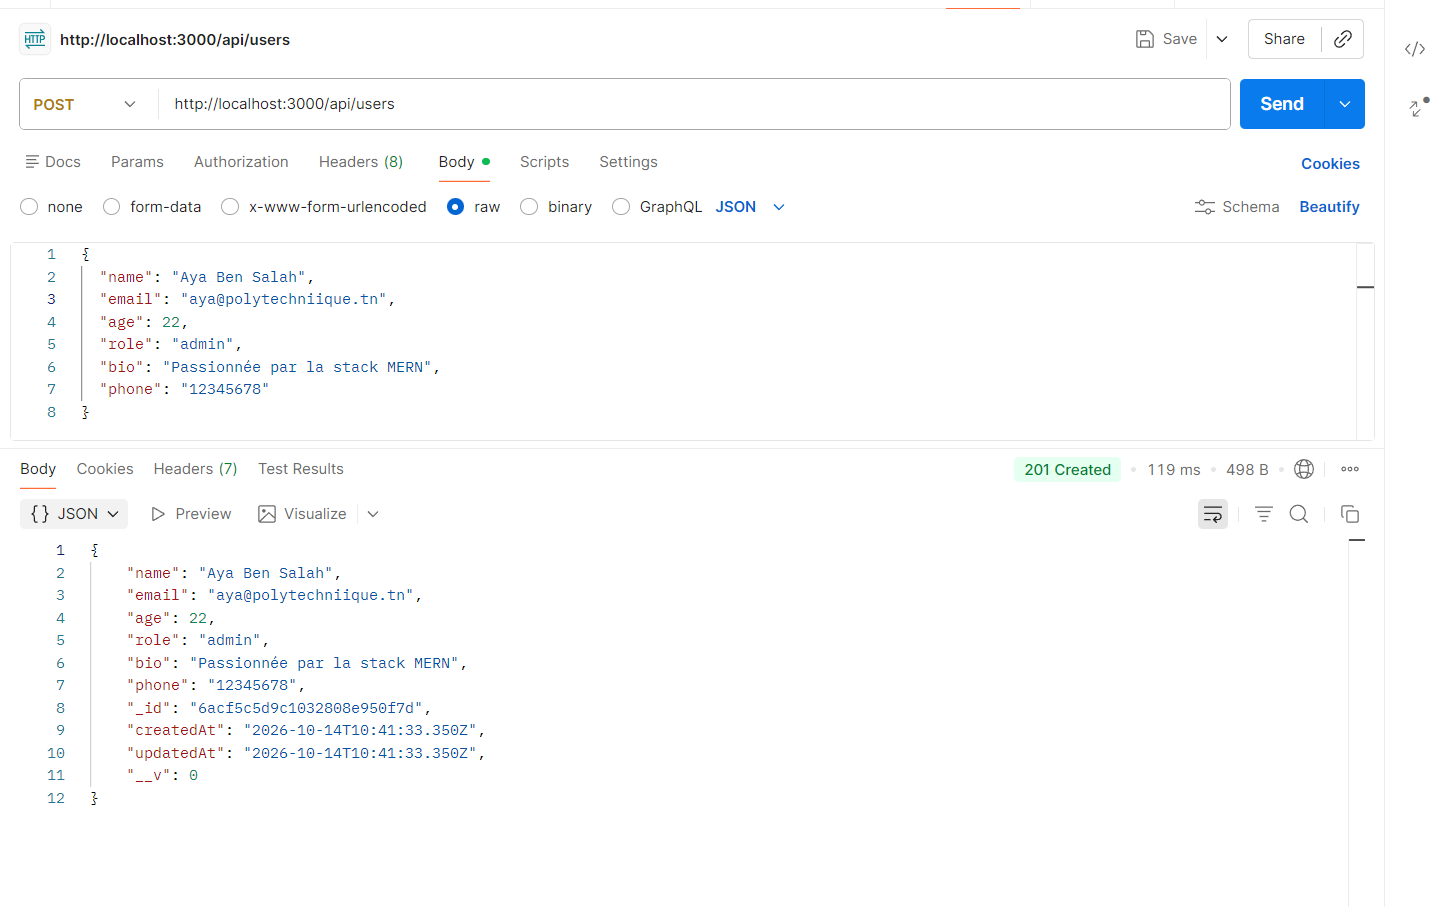
\includegraphics[width=0.78\textwidth]{postmanTP4-4.png}
    \caption{GET /api/users/profile -- 200 OK (Authorization: Bearer <token>)}
    \vspace{0.1cm}
    \small \textit{Description :} Même route avec l'en-tête \texttt{Authorization: Bearer <token>}. Le middleware \texttt{protect} extrait et vérifie le JWT, récupère l'utilisateur en base (sans le champ \texttt{password} grâce à \texttt{.select('-password')}), l'injecte dans \texttt{req.user} et passe la main au contrôleur.
\end{figure}

\clearpage
\subsection{Création d'un article protégé -- 201 Created}

\begin{figure}[htbp]
    \centering
    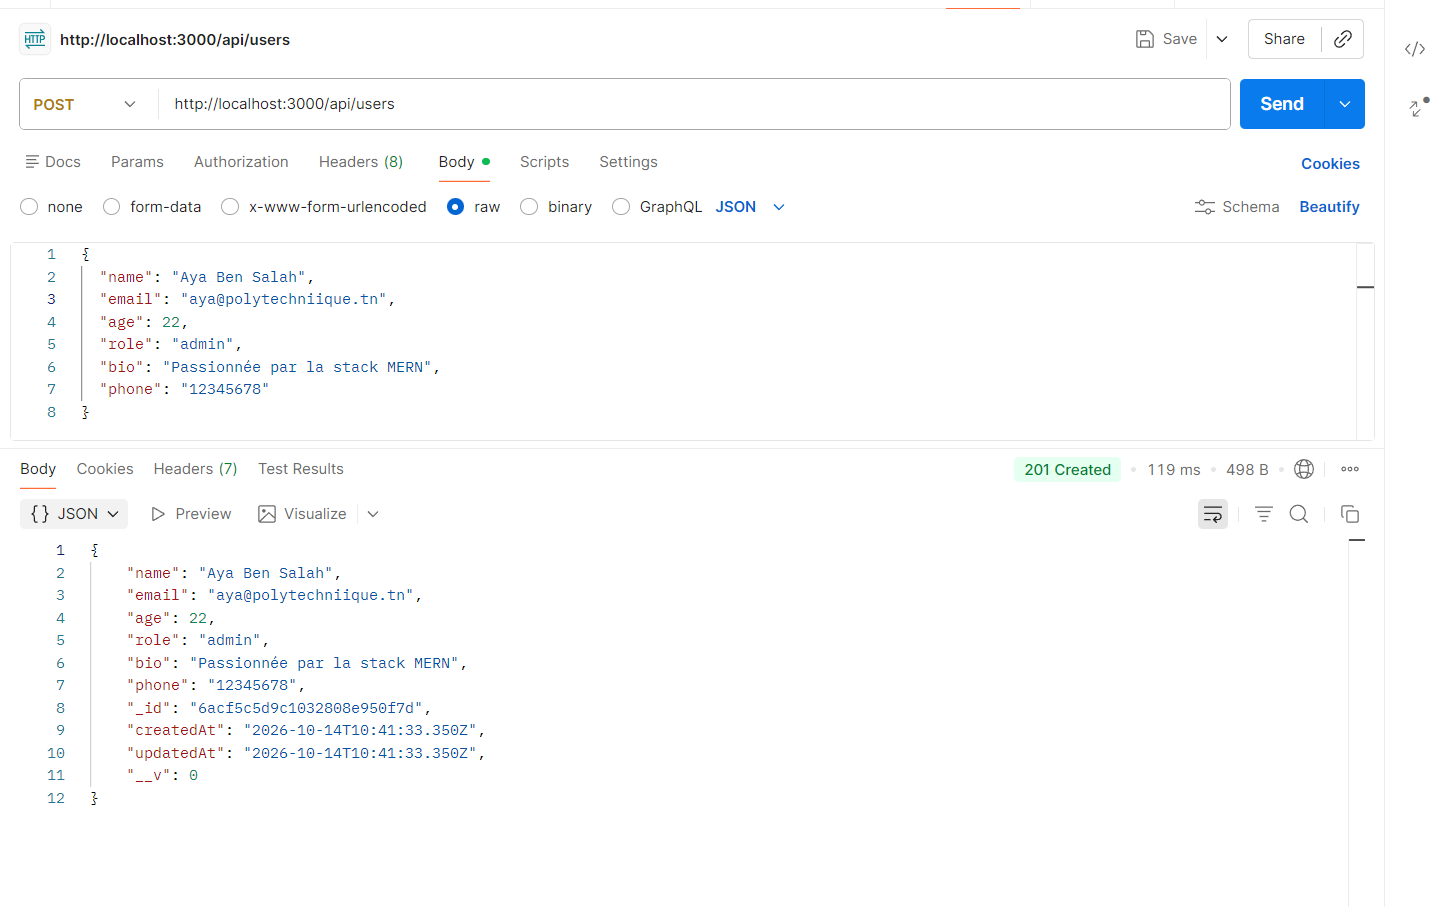
\includegraphics[width=0.78\textwidth]{postmanTP4-5.png}
    \caption{POST /api/articles -- 201 Created (auteur extrait du JWT)}
    \vspace{0.1cm}
    \small \textit{Description :} Création d'un article en fournissant uniquement \texttt{title} et \texttt{content}. L'auteur est fixé par le serveur depuis \texttt{req.user.\_id} extrait du token — aucune usurpation d'identité n'est possible. La réponse inclut l'objet auteur peuplé via \texttt{.populate()}.
\end{figure}

\clearpage
\subsection{Refus RBAC -- 403 Forbidden (compte simple)}

\begin{figure}[htbp]
    \centering
    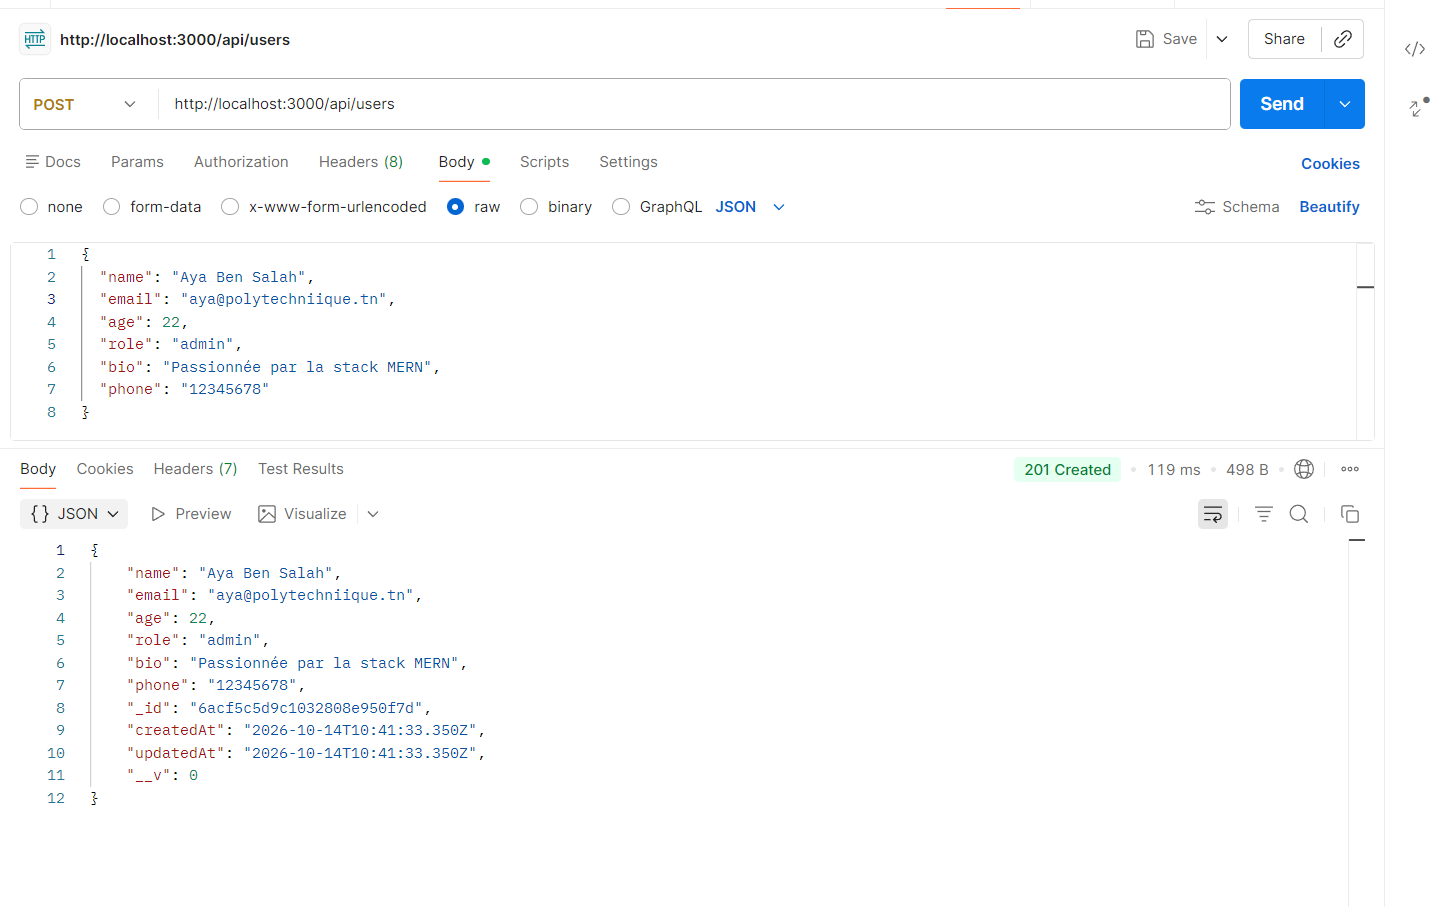
\includegraphics[width=0.78\textwidth]{postmanTP4-6.png}
    \caption{GET /api/users -- 403 Forbidden (role: user, adminOnly échoue)}
    \vspace{0.1cm}
    \small \textit{Description :} Tentative d'accès à la liste des utilisateurs (route \texttt{protect + adminOnly}) avec un token de role \texttt{"user"}. Le middleware \texttt{adminOnly} détecte que \texttt{req.user.role !== 'admin'} et bloque avec \textbf{403 Forbidden} : \texttt{"Acces refuse : droits administrateur requis"}.
\end{figure}

\clearpage
\subsection{Exercice 1 : Mise à jour sécurisée du mot de passe -- 200 OK}

\begin{figure}[htbp]
    \centering
    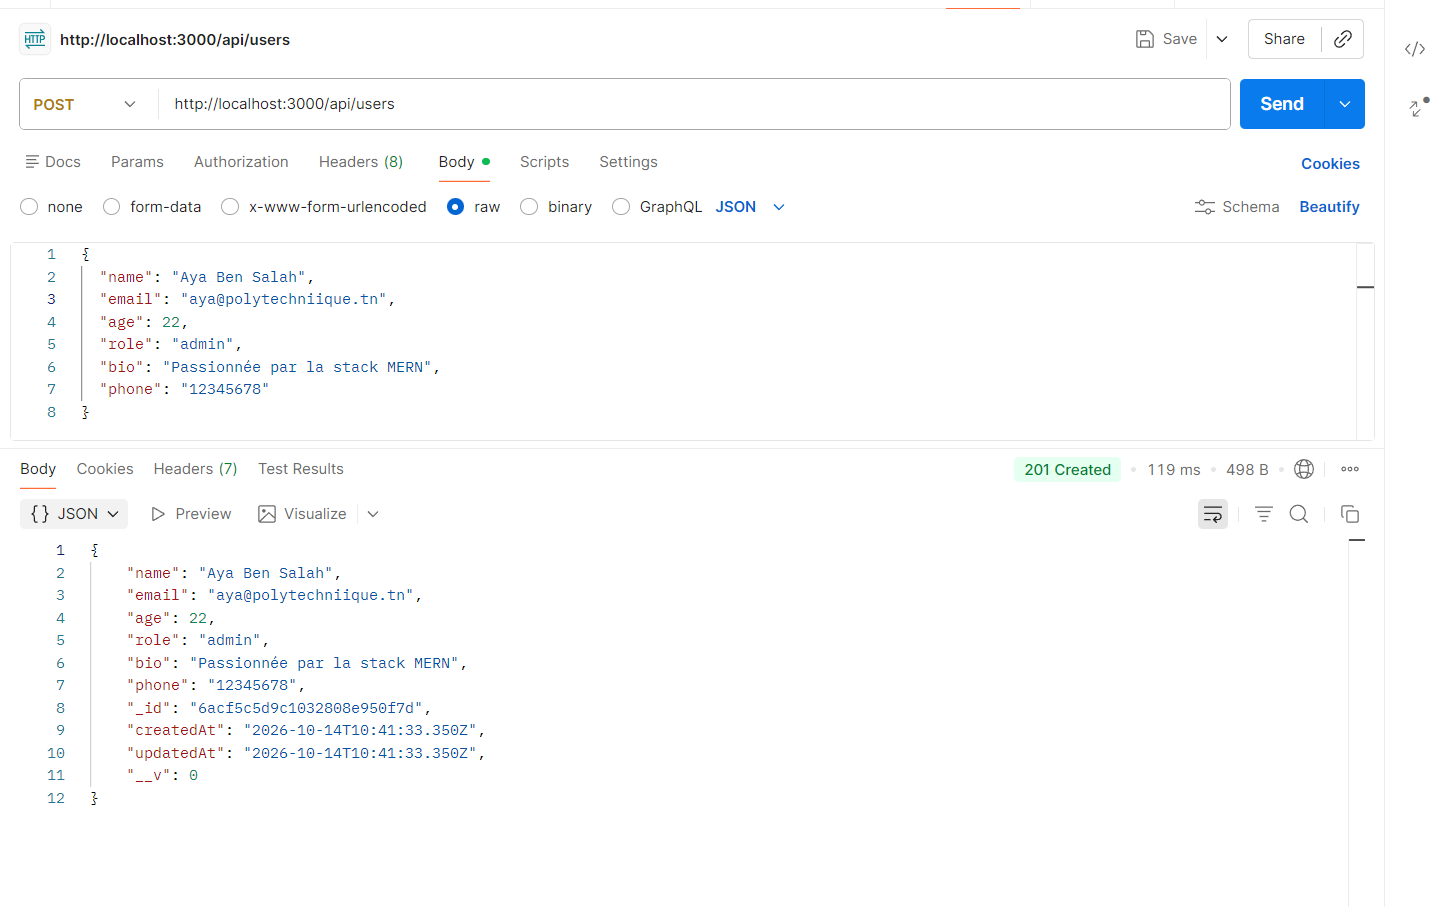
\includegraphics[width=0.78\textwidth]{postmanTP4-7.png}
    \caption{PUT /api/users/update-password -- 200 OK (Exercice 1)}
    \vspace{0.1cm}
    \small \textit{Description :} L'utilisateur connecté soumet \texttt{oldPassword} et \texttt{newPassword}. Le contrôleur vérifie l'ancien mot de passe avec \texttt{bcrypt.compare()}, génère un nouveau sel, hache le nouveau mot de passe et sauvegarde. Réponse \textbf{200 OK} : \texttt{"Mot de passe mis a jour avec succes"}.
\end{figure}

\clearpage
\subsection{Exercice 2 : Articles personnels \& protection contre l'escalade de rôle}

\begin{figure}[htbp]
    \centering
    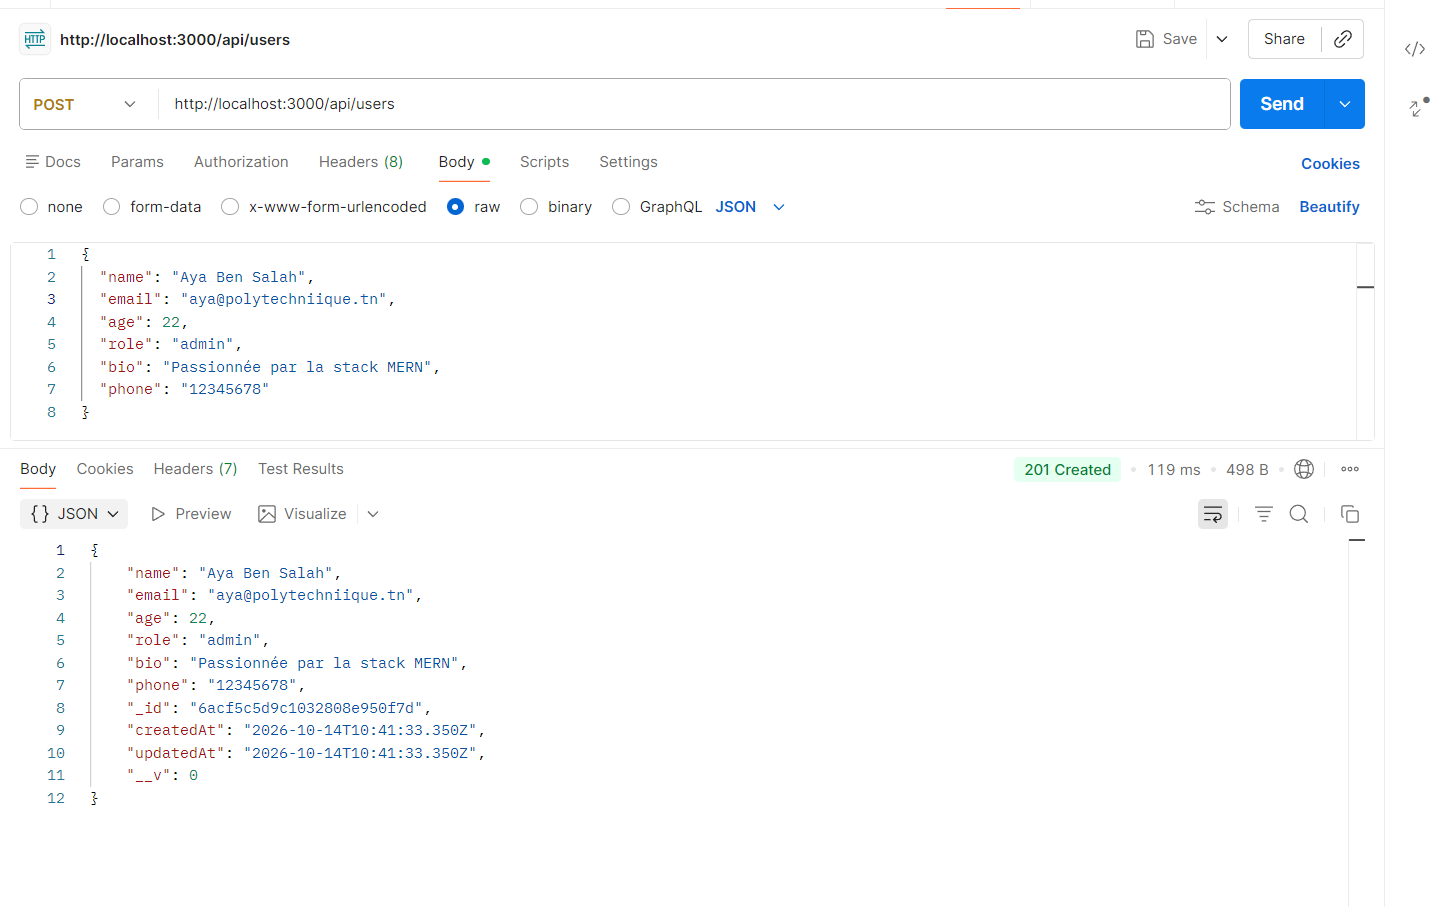
\includegraphics[width=0.78\textwidth]{postmanTP4-8.png}
    \caption{GET /api/articles/my-articles -- 200 OK + protection escalade (Exercice 2)}
    \vspace{0.1cm}
    \small \textit{Description :} \textbf{(a)} Route \texttt{GET /api/articles/my-articles} : filtre les articles dont \texttt{author === req.user.\_id} — seuls les articles de l'utilisateur connecté sont retournés. \textbf{(b)} Tentative d'inscription avec \texttt{"role":"admin"} dans le body : le contrôleur force \texttt{role = 'user'} — le rôle reçu est bien \texttt{"user"}, prouvant la protection contre l'escalade de privilèges.
\end{figure}

\newpage
\section{Code Source Intégral du Projet}

\subsection{Middleware de sécurité : \texttt{src/middlewares/authMiddleware.js}}
\begin{lstlisting}
const jwt = require('jsonwebtoken');
const User = require('../models/userModel');

// 1. Protection des routes privees : verifie la validite du JWT
const protect = async (req, res, next) => {
  let token;
  if (
    req.headers.authorization &&
    req.headers.authorization.startsWith('Bearer ')
  ) {
    try {
      token = req.headers.authorization.split(' ')[1];
      const decoded = jwt.verify(token, process.env.JWT_SECRET);
      req.user = await User.findById(decoded.id).select('-password');
      if (!req.user) {
        return res.status(401).json({ message: 'Non autorise, utilisateur introuvable' });
      }
      return next();
    } catch (err) {
      // Exercice 3 : Gestion explicite de l'expiration du token
      if (err.name === 'TokenExpiredError') {
        return res.status(401).json({
          message: 'Votre session a expire, veuillez vous reconnecter'
        });
      }
      return res.status(401).json({ message: 'Non autorise, token invalide ou expire' });
    }
  }
  return res.status(401).json({ message: 'Non autorise, aucun token fourni' });
};

// 2. Controle d'acces base sur les roles (RBAC) : reserve aux admins
const adminOnly = (req, res, next) => {
  if (req.user && req.user.role === 'admin') {
    return next();
  }
  return res.status(403).json({ message: 'Acces refuse : droits administrateur requis' });
};

module.exports = { protect, adminOnly };
\end{lstlisting}

\subsection{Contrôleur utilisateurs enrichi : \texttt{src/controllers/userController.js}}
\begin{lstlisting}
const bcrypt = require('bcryptjs');
const jwt = require('jsonwebtoken');
const User = require('../models/userModel');

const generateToken = (id, role) => {
  return jwt.sign({ id, role }, process.env.JWT_SECRET, { expiresIn: '1d' });
};

// POST /api/users/register
const registerUser = async (req, res) => {
  try {
    const { name, email, password, age } = req.body;
    if (!name || !email || !password) {
      return res.status(400).json({ message: 'Nom, email et mot de passe requis' });
    }
    const userExists = await User.findOne({ email });
    if (userExists) {
      return res.status(409).json({ message: 'Cet email est deja utilise' });
    }
    const salt = await bcrypt.genSalt(10);
    const hashedPassword = await bcrypt.hash(password, salt);
    // Exercice 2 : Protection contre escalade de privileges
    const user = await User.create({
      name, email, password: hashedPassword, age, role: 'user'
    });
    res.status(201).json({
      _id: user._id, name: user.name, email: user.email,
      role: user.role, token: generateToken(user._id, user.role)
    });
  } catch (err) {
    if (err.name === 'ValidationError') return res.status(400).json({ message: err.message });
    res.status(500).json({ message: err.message });
  }
};

// POST /api/users/login
const loginUser = async (req, res) => {
  try {
    const { email, password } = req.body;
    if (!email || !password) {
      return res.status(400).json({ message: 'Email et mot de passe requis' });
    }
    const user = await User.findOne({ email });
    if (!user) return res.status(401).json({ message: 'Identifiants invalides' });
    const isMatch = await bcrypt.compare(password, user.password);
    if (!isMatch) return res.status(401).json({ message: 'Identifiants invalides' });
    res.status(200).json({
      _id: user._id, name: user.name, email: user.email,
      role: user.role, token: generateToken(user._id, user.role)
    });
  } catch (err) {
    res.status(500).json({ message: err.message });
  }
};

// GET /api/users/profile
const getUserProfile = async (req, res) => {
  res.status(200).json(req.user);
};

// GET /api/users (Admin)
const getAllUsers = async (req, res) => {
  try {
    const users = await User.find().select('-password');
    res.status(200).json(users);
  } catch (err) {
    res.status(500).json({ message: err.message });
  }
};

// PUT /api/users/update-password (Exercice 1)
const updatePassword = async (req, res) => {
  try {
    const { oldPassword, newPassword } = req.body;
    if (!oldPassword || !newPassword) {
      return res.status(400).json({ message: 'Ancien et nouveau mot de passe requis' });
    }
    const user = await User.findById(req.user._id);
    const isMatch = await bcrypt.compare(oldPassword, user.password);
    if (!isMatch) {
      return res.status(401).json({ message: 'Ancien mot de passe incorrect' });
    }
    const salt = await bcrypt.genSalt(10);
    user.password = await bcrypt.hash(newPassword, salt);
    await user.save();
    res.status(200).json({ message: 'Mot de passe mis a jour avec succes' });
  } catch (err) {
    res.status(500).json({ message: err.message });
  }
};

// PUT /api/users/:id/role (Exercice 2 : elevation de role, admin seulement)
const updateUserRole = async (req, res) => {
  try {
    const { role } = req.body;
    if (!role || !['user', 'admin'].includes(role)) {
      return res.status(400).json({ message: "Role invalide. Valeurs : 'user', 'admin'" });
    }
    const user = await User.findByIdAndUpdate(
      req.params.id, { role }, { new: true, runValidators: true }
    ).select('-password');
    if (!user) return res.status(404).json({ message: 'Utilisateur non trouve' });
    res.status(200).json({ message: `${user.name} est maintenant ${user.role}`, user });
  } catch (err) {
    if (err.name === 'CastError') {
      return res.status(400).json({ message: 'Identifiant invalide (format ObjectId attendu)' });
    }
    res.status(500).json({ message: err.message });
  }
};

module.exports = { registerUser, loginUser, getUserProfile, getAllUsers, updatePassword, updateUserRole };
\end{lstlisting}

\subsection{Contrôleur articles sécurisé : \texttt{src/controllers/articleController.js}}
\begin{lstlisting}
const Article = require('../models/articleModel');

// GET /api/articles
const getAllArticles = async (req, res) => {
  try {
    const articles = await Article.find().populate('author', 'name email role');
    res.status(200).json(articles);
  } catch (err) { res.status(500).json({ message: err.message }); }
};

// GET /api/articles/my-articles (Exercice 2)
const getMyArticles = async (req, res) => {
  try {
    const articles = await Article.find({ author: req.user._id })
      .populate('author', 'name email role');
    res.status(200).json(articles);
  } catch (err) { res.status(500).json({ message: err.message }); }
};

// POST /api/articles (Creation protegee)
const createArticle = async (req, res) => {
  try {
    const { title, content } = req.body;
    if (!title || !content) {
      return res.status(400).json({ message: 'Titre et contenu obligatoires' });
    }
    // L'auteur est extrait du token : usurpation impossible !
    const newArticle = await Article.create({ title, content, author: req.user._id });
    const populated = await newArticle.populate('author', 'name email role');
    res.status(201).json(populated);
  } catch (err) { res.status(500).json({ message: err.message }); }
};

// PUT /api/articles/:id (Modification : auteur ou admin)
const updateArticle = async (req, res) => {
  try {
    const article = await Article.findById(req.params.id);
    if (!article) return res.status(404).json({ message: 'Article non trouve' });
    if (
      article.author.toString() !== req.user._id.toString() &&
      req.user.role !== 'admin'
    ) {
      return res.status(403).json({ message: "Action interdite : vous n'etes pas l'auteur" });
    }
    article.title = req.body.title || article.title;
    article.content = req.body.content || article.content;
    const updated = await article.save();
    const populated = await updated.populate('author', 'name email role');
    res.status(200).json(populated);
  } catch (err) {
    if (err.name === 'CastError') return res.status(400).json({ message: 'Identifiant invalide' });
    res.status(500).json({ message: err.message });
  }
};

// DELETE /api/articles/:id (Suppression : auteur ou admin)
const deleteArticle = async (req, res) => {
  try {
    const article = await Article.findById(req.params.id);
    if (!article) return res.status(404).json({ message: 'Article non trouve' });
    if (
      article.author.toString() !== req.user._id.toString() &&
      req.user.role !== 'admin'
    ) {
      return res.status(403).json({ message: "Action interdite : vous n'etes pas l'auteur" });
    }
    await Article.findByIdAndDelete(req.params.id);
    res.status(200).json({ message: 'Article supprime avec succes', id: req.params.id });
  } catch (err) {
    if (err.name === 'CastError') return res.status(400).json({ message: 'Identifiant invalide' });
    res.status(500).json({ message: err.message });
  }
};

module.exports = { getAllArticles, getArticleById: async (req, res) => {
  try {
    const article = await Article.findById(req.params.id).populate('author', 'name email role');
    if (!article) return res.status(404).json({ message: 'Article non trouve' });
    res.status(200).json(article);
  } catch (err) {
    if (err.name === 'CastError') return res.status(400).json({ message: 'Identifiant invalide' });
    res.status(500).json({ message: err.message });
  }
}, createArticle, getMyArticles, updateArticle, deleteArticle };
\end{lstlisting}

\subsection{Routeur utilisateurs : \texttt{src/routes/userRoutes.js}}
\begin{lstlisting}
const express = require('express');
const router = express.Router();
const {
  registerUser, loginUser, getUserProfile,
  getAllUsers, updatePassword, updateUserRole
} = require('../controllers/userController');
const { protect, adminOnly } = require('../middlewares/authMiddleware');

router.post('/register', registerUser);
router.post('/login', loginUser);
// Exercice 1 : Mise a jour securisee du mot de passe
router.put('/update-password', protect, updatePassword);
// Profil prive
router.get('/profile', protect, getUserProfile);
// Exercice 2 : Elevation de role (admin uniquement)
router.put('/:id/role', protect, adminOnly, updateUserRole);
// Liste des utilisateurs (admin uniquement)
router.get('/', protect, adminOnly, getAllUsers);

module.exports = router;
\end{lstlisting}

\subsection{Routeur articles : \texttt{src/routes/articleRoutes.js}}
\begin{lstlisting}
const express = require('express');
const router = express.Router();
const {
  getAllArticles, getArticleById,
  createArticle, getMyArticles,
  updateArticle, deleteArticle
} = require('../controllers/articleController');
const { protect } = require('../middlewares/authMiddleware');

// Consultation publique
router.get('/', getAllArticles);
// Exercice 2 : Route des articles personnels (avant /:id pour eviter conflit)
router.get('/my-articles', protect, getMyArticles);
// Consultation par ID
router.get('/:id', getArticleById);
// Operations d'ecriture protegees
router.post('/', protect, createArticle);
router.put('/:id', protect, updateArticle);
router.delete('/:id', protect, deleteArticle);

module.exports = router;
\end{lstlisting}

\section*{Conclusion}
Ce TP 4 finalise la couche de sécurité de notre API MERN. Grâce à \textbf{bcryptjs}, les mots de passe ne sont jamais stockés en clair : seul leur empreinte irréversible est persiste. Le \textbf{JWT} permet une authentification \textit{stateless} scalable : le serveur n'a pas besoin de session. Le middleware \texttt{protect} centralise la vérification cryptographique, et \texttt{adminOnly} applique le RBAC. Les exercices renforcent la sécurité : changement de mot de passe authentifié, filtrage des ressources personnelles, blocage de l'escalade de privilèges et gestion fine de l'expiration des tokens.

\end{document}
